%\subsection{Scheme Comparison}
%\label{subsec:scheme-comparison}

We summarize and compare TFHE, BFV, CKKS, and BGV as follows:

\begin{comment}
\clearpage



\end{comment}

\captionsetup{justification=raggedright,singlelinecheck=false,labelfont=bf}

\begin{table}[h]
\begin{tabular}{|c||l|}
\hline
&\textbf{Hard Problem Basis}\\\hline\hline
\textbf{TFHE}&LWE\\\hline
\textbf{BFV}&\\
\textbf{CKKS}&RLWE\\
\textbf{BGV}&\\\hline
\end{tabular}
\caption{\textbf{Hard Problem Basis}}
\end{table}

\begin{table}[h]
\begin{tabular}{|c||l|}
\hline
&\textbf{Unit Data Type}\\\hline\hline
\textbf{TFHE}&Vector\\\hline
\textbf{BFV}&\\
\textbf{CKKS}&Polynomial\\
\textbf{BGV}&\\\hline
\end{tabular}
\caption{\textbf{Unit Data Type}}
\end{table}

\begin{table}[h]
\begin{tabular}{|c||l|}
\hline
&\multicolumn{1}{c|}{\textbf{Plaintext}}\\\hline\hline
\textbf{TFHE}&Number $m \in \mathbb{Z}_t$ \text{ } \textcolor{red}{ \# $t$ is a power of 2}\\\hline
\textbf{BFV}&Polynomial $M \in \mathbb{Z}_t[X]/X^n+1$ \text{ } \textcolor{red}{ \# $t$ is a prime, and $n$ is a power of 2}\\\hline
\textbf{CKKS}&Polynomial $M \in \mathbb{R}[X]/X^n+1$ \text{ }\textcolor{red}{ \# $n$ is a power of 2}\\\hline
\textbf{BGV}&Polynomial $M \in \mathbb{Z}_t[X]/X^n+1$ \text{ } \textcolor{red}{ \# $t$ is a prime, and $n$ is a power of 2}\\\hline
\end{tabular}
\caption{\textbf{Plaintext}}
\end{table}

\begin{table}[h]
\begin{tabular}{|c||l|}
\hline
&\multicolumn{1}{c|}{\textbf{Secret Key}}\\\hline\hline
\textbf{TFHE}&Vector $\vec{s} \xleftarrow{\$} \mathbb{Z}_2^k$ \text{ } \textcolor{red}{ \# $\$$ is a uniform random distribution}\\\hline
\textbf{BFV}&\\
\textbf{CKKS}&Polynomial $S \xleftarrow{\$} \mathbb{Z}_3[X]/X^n+1$, where we set $\mathbb{Z}_3 = \{-1, 0, 1\}$\\
\textbf{BGV}&\\\hline
\end{tabular}
\caption{\textbf{Secret Key}}
\end{table}

\begin{table}[h]
\begin{tabular}{|c||l|}
\hline
&\multicolumn{1}{c|}{\textbf{Ciphertext}}\\\hline\hline
\textbf{TFHE}&(Vector $\vec{a}$, Number $b$) = $(\vec{a} \xleftarrow{\$} \mathbb{Z}_q^k$, $\text{ } b \in \mathbb{Z}_q)$ \text{ } \textcolor{red}{ \# $q \gg t$, and $t$ divides $q$}\\\hline
\textbf{BFV}&\\
\textbf{CKKS}&(Polynomial $A, B$) = $(A \xleftarrow{\$} \mathbb{Z}_q[X]/X^n+1$, \text{ }  $B \in \mathbb{Z}_q[X]/X^n+1)$ \text{ } \textcolor{red}{ \# $q \gg t$}\\
\textbf{BGV}&\\\hline
\end{tabular}
\caption{\textbf{Ciphertext}}
\end{table}


\begin{table}[h]
\begin{tabular}{|c||l|}
\hline
&\multicolumn{1}{c|}{\textbf{Noise}}\\\hline\hline
\textbf{TFHE}&Number $e \xleftarrow{\chi} \mathbb{Z}_q$ \text{ } \textcolor{red}{ \# $\chi$ is a Gaussian random distribution}\\\hline
\textbf{BFV}&\\
\textbf{CKKS}&Polynomial $E \xleftarrow{\chi} \mathbb{Z}_q[X]/X^n+1$\\
\textbf{BGV}&\\\hline
\end{tabular}
\caption{\textbf{Noise}}
\end{table}


\begin{table}[h]
\begin{tabular}{|c||l|}
\hline
&\multicolumn{1}{c|}{\textbf{Scaling Factor}}\\\hline\hline
\textbf{TFHE}&Used for $\Delta m$, \text{ } where $\Delta = \dfrac{q}{t}$ \text{ } \textcolor{red}{\# $t$ divides $q$}\\\hline
\textbf{BFV}&Used for $\Delta M$, \text{ } where $\Delta = \left\lfloor\dfrac{q}{t}\right\rfloor$  \text{ } \textcolor{red}{\# $t$ is a prime}\\\hline
\textbf{CKKS}&Used for $\Delta M$, \text{ } where $\Delta \cdot ||M||_\infty \ll q_0$\\
& \text{ } \textcolor{red}{\# $q_0$ is the lowest multiplicative level's ciphertext modulus}\\\hline
\textbf{BGV}&Used for $\Delta E$, \text{ } where $\Delta = t$ \text{ } \textcolor{red}{ \#$t$ is a prime}\\\hline
\end{tabular}
\caption{\textbf{Scaling Factor}}
\end{table}


\begin{table}[h]
\begin{tabular}{|c||l|}
\hline
&\multicolumn{1}{c|}{\textbf{Encryption}}\\\hline\hline
\textbf{TFHE}&$(\vec{a}, b)$ \text{ } where $\vec{a} \xleftarrow{\$} \mathbb{Z}_q^k$, $\text{ } b = \Delta m + e - a\cdot s \bmod q$, \text{ } $e \xleftarrow{\chi} \mathbb{Z}_q$\\
&\text{ } \text{ } \textcolor{red}{ \# After using $e$ each time, throw it away}\\\hline
\textbf{BFV}&$(A, B)$ \text{ } where $A \xleftarrow{\$} \mathbb{Z}_q[X] / (X^n + 1)$, $\text{ } B = \Delta M + E - A\cdot S \bmod q$, \text{ } $E \xleftarrow{\chi} \mathbb{Z}_q$\\
\textbf{CKKS}&\text{ } \text{ }\textcolor{red}{ \# After using $E$ each time, throw it away}\\\hline
\textbf{BGV}&$(A, B)$ \text{ } where $A \xleftarrow{\$} \mathbb{Z}_q[X] / (X^n + 1)$, $\text{ } B = M + \Delta E - A\cdot S \bmod q$, \text{ } $E \xleftarrow{\chi} \mathbb{Z}_q$\\
&\text{ } \text{ }\textcolor{red}{ \# After using $E$ each time, throw it away}\\\hline
\end{tabular}
\caption{\textbf{Encryption}}
\end{table}

\begin{table}[h]
\begin{tabular}{|c||l|}
\hline
&\multicolumn{1}{c|}{\textbf{Cryptographic Relation}}\\\hline\hline
\textbf{TFHE}&$b + a\cdot s = \Delta m + e \pmod q$, \text{ } where $\Delta = \dfrac{q}{t}$  \text{ } \textcolor{red}{\# $t$ divides $q$}\\\hline
\textbf{BFV}&$B + A\cdot S = \Delta M + E \pmod q$, \text{ } where $\Delta = \left\lfloor\dfrac{q}{t}\right\rfloor$ \text{ } \textcolor{red}{\# $t$ is a prime}\\\hline
\textbf{CKKS}&$B + A\cdot S = \Delta M + E \pmod q$, \text{ } where $\Delta \cdot ||M||_\infty \ll q_0$\\
& \text{ } \textcolor{red}{\# $q_0$ is the lowest multiplicative level's ciphertext modulus}\\\hline
\textbf{BGV}&$B + A\cdot S = M + \Delta E \pmod q$, \text{ } where $\Delta = t$  \text{ } \textcolor{red}{\# $t$ is a prime}\\\hline
\end{tabular}
\caption{\textbf{Cryptographic Relation}}
\end{table}


\begin{table}[h]
\begin{tabular}{|c||l|}
\hline
&\multicolumn{1}{c|}{\textbf{Decryption Formula}}\\\hline\hline
\textbf{TFHE}&$m = \left\lceil\dfrac{(b + a\cdot s \bmod q)}{\Delta}\right\rfloor \bmod t$\\
&$\textcolor{white}{m} = \left\lceil\dfrac{(\Delta m + e)}{\Delta}\right\rfloor \bmod t$ \text{ } \textcolor{red}{ \# $e$ gets eliminated if $e < \dfrac{\Delta}{2}$}\\\hline
\textbf{BFV}&$M = \left\lceil\dfrac{(B + A\cdot S \bmod q)}{\Delta}\right\rfloor  \bmod t$\\
&$\textcolor{white}{M} = \left\lceil\dfrac{(\Delta M + E)}{\Delta}\right\rfloor  \bmod t$ \text{ } \textcolor{red}{ \# $E$ gets eliminated if $||E||_\infty < \dfrac{\Delta}{2}$}\\\hline
\textbf{CKKS}&$M = \left\lceil\dfrac{(B + A\cdot S \bmod q)}{\Delta}\right\rfloor_{\frac{1}{\Delta}}$\\
&$\textcolor{white}{M} = \left\lceil\dfrac{\Delta M + E}{\Delta}\right\rfloor_{\frac{1}{\Delta}}$ \text{ } \textcolor{red}{ \# The final noise remains as $\dfrac{E}{\Delta}$ (increase $\Delta$ to reduce it)}\\\hline
\textbf{BGV}&$M = (B + A\cdot S \bmod q) \bmod t$\\
&$\textcolor{white}{M} = (M + \Delta E) \bmod t$ \text{ } \textcolor{red}{ \# $E$ gets eliminated if $\Delta E < q$}\\\hline
\end{tabular}
\caption{\textbf{Decryption Formula}}
\end{table}

\begin{table}[h]
\begin{tabular}{|c||l|}
\hline
&\multicolumn{1}{c|}{\textbf{Ciphertext Modulus}}\\\hline\hline
\textbf{TFHE}&A single number $q$ \text{ } \textcolor{red}{ \# $q \gg t$, and $t$ divides $q$}\\\hline
\textbf{BFV}&A single number $q$ \text{ } \textcolor{red}{ \# $q \gg t$}\\\hline
\textbf{CKKS}&An $L$-multiplicative-level modulus chain $\{q_0, q_1, \cdots, q_L\}$\\
& \text{ } \textcolor{red}{ \# each $q_i = \prod\limits_{j=0}^{l}w_j$, and each $w_j$ is a CRT modulus}\\
&\text{ } \text{ } \text{ } \textcolor{red}{ having the property: $w_0 \gg \Delta \cdot ||M||_{\infty}, \text{ } w_j \approx \Delta$ (for $1 \leq j \leq L$)}\\\hline
\textbf{BGV}&An $L$-multiplicative-level modulus chain $\{q_0, q_1, \cdots, q_L\}$\\
&\text{ } \textcolor{red}{ \# each $q_i = \prod\limits_{j=0}^{l}w_j$, and each $w_j$ is a CRT modulus}\\
&\text{ } \text{ } \text{ } \textcolor{red}{ having the property: $w_0 \equiv w_1 \equiv \cdots \equiv w_L \bmod t$}\\\hline
\end{tabular}
\caption{\textbf{Ciphertext Modulus}}
\end{table}



\begin{table}[h]
\begin{tabular}{|c||l|}
\hline
&\multicolumn{1}{c|}{\textbf{Ciphertext-to-Ciphertext Addition}}\\\hline\hline
\textbf{TFHE}&- Ciphertext $\textsf{LWE}_{\vec{s}, \sigma}(\Delta m_1) = (\vec{a}_1, b_1) = (a_{1,0}, a_{1, 1}, \cdots, a_{1, k-1}, b_1) \bmod q$\\
&- Ciphertext $\textsf{LWE}_{\vec{s}, \sigma}(\Delta m_2) = (\vec{a}_2, b_2) = (a_{2,0}, a_{2, 1}, \cdots, a_{2, k-1}, b_2) \bmod q$\\
&$\textsf{LWE}_{\vec{s}, \sigma}(\Delta (m_1 + m_2)) = (\vec{a}_1+\vec{a}_2, b_1+b_2) \bmod q$\\\hline
\textbf{BFV}&- Ciphertext $\textsf{RLWE}_{S, \sigma}(\Delta M_1) = (A_1, B_1) \bmod q$\\
&- Ciphertext $\textsf{RLWE}_{S, \sigma}(\Delta M_2) = (A_2, B_2) \bmod q$\\
&$\textsf{RLWE}_{S, \sigma}(\Delta (M_1 + M_2)) =(A_1+A_2,B_1+B_2) \bmod q$\\\hline
\textbf{CKKS}&- Ciphertext $\textsf{RLWE}_{S, \sigma}(\Delta M_1) = (A_1, B_1) \bmod q_l$\\
&- Ciphertext $\textsf{RLWE}_{S, \sigma}(\Delta M_2) = (A_2, B_2) \bmod q_l$\\
&$\textsf{RLWE}_{S, \sigma}(\Delta (M_1 + M_2)) =(A_1+A_2,B_1+B_2) \bmod q_l$\\\hline
\textbf{BGV}&- Ciphertext $\textsf{RLWE}_{S, \sigma}(M_1) = (A_1, B_1) \bmod q_l$\\
&- Ciphertext $\textsf{RLWE}_{S, \sigma}(M_2) = (A_2, B_2) \bmod q_l$\\
&$\textsf{RLWE}_{S, \sigma}(M_1 + M_2) =(A_1+A_2,B_1+B_2) \bmod q_l$\\\hline
\end{tabular}
\caption{\textbf{Ciphertext-to-Ciphertext Addition}}
\end{table}

\begin{table}[h]
\begin{tabular}{|c||l|}
\hline
&\multicolumn{1}{c|}{\textbf{Ciphertext-to-Plaintext Addition}}\\\hline\hline
\textbf{TFHE}&- Ciphertext $\textsf{LWE}_{\vec{s}, \sigma}(\Delta m_1) = (\vec{a}_1, b_1) = (a_{1,0}, a_{1, 1}, \cdots, a_{1, k-1}, b_1) \bmod q$\\
&- Plaintext number $c \in \mathbb{Z}_t$\\
&$\textsf{LWE}_{\vec{s}, \sigma}(\Delta (m_1 + c)) = (\vec{a}_1, b_1+\Delta c) \bmod q$\\\hline
\textbf{BFV}&- Ciphertext $\textsf{RLWE}_{S, \sigma}(\Delta M_1) = (A_1, B_1) \bmod q$\\
&- Plaintext polynomial $C \in \mathbb{Z}_t[X]/(X^n + 1)$\\
&$\textsf{RLWE}_{S, \sigma}(\Delta (M_1 + C)) =(A_1,B_1+\Delta C) \bmod q$\\\hline
\textbf{CKKS}&- Ciphertext $\textsf{RLWE}_{S, \sigma}(\Delta M_1) = (A_1, B_1)  \bmod q_l$\\
&- Plaintext polynomial $C \in \mathbb{R}[X]/(X^n + 1)$\\
&$\textsf{RLWE}_{S, \sigma}(\Delta (M_1 + C)) =(A_1,B_1+\Delta C) \bmod q_l$\\\hline
\textbf{BGV}&- Ciphertext $\textsf{RLWE}_{S, \sigma}(M_1) = (A_1, B_1) \bmod q_l$\\
&- Plaintext polynomial $C \in \mathbb{Z}_t[X]/(X^n + 1)$\\
&$\textsf{RLWE}_{S, \sigma}(M_1 + C) =(A_1,B_1+C) \bmod q_l$\\\hline
\end{tabular}
\caption{\textbf{Ciphertext-to-Plaintext Addition}}
\end{table}

\begin{table}[h]
\begin{tabular}{|c||l|}
\hline
&\multicolumn{1}{c|}{\textbf{Ciphertext-to-Plaintext Multiplication}}\\\hline\hline
\textbf{TFHE}&- Ciphertext $\textsf{LWE}_{\vec{s}, \sigma}(\Delta m_1) = (\vec{a}_1, b_1) = (a_{1,0}, a_{1, 1}, \cdots, a_{1, k-1}, b_1) \bmod q$\\
&- Plaintext number $c \in \mathbb{Z}_t$\\
&$\textsf{LWE}_{\vec{s}, \sigma}(\Delta (m_1 \cdot c)) = (\vec{a}_1 \cdot c, \text{ } b_1 \cdot c) \bmod q$\\\hline
\textbf{BFV}&- Ciphertext $\textsf{RLWE}_{S, \sigma}(\Delta M_1) = (A_1, B_1) \bmod q$\\
&- Plaintext polynomial $C \in \mathbb{Z}_t[X]/(X^n + 1)$\\
&$\textsf{RLWE}_{S, \sigma}(\Delta (M_1 \cdot C)) =(A_1 \cdot C, \text{ } B_1 \cdot C)$\\\hline
\textbf{CKKS}&- Ciphertext $\textsf{RLWE}_{S, \sigma}(\Delta M_1) = (A_1, B_1)  \bmod q_l$\\
&- Plaintext polynomial $C \in \mathbb{R}/(X^n + 1)$\\
&1. \underline{Basic Multiplication}\\
&\textcolor{white}{1. } $\textsf{ct} = \textsf{RLWE}_{S, \sigma}(\Delta^2 (M_1 \cdot C)) =(A_1 \cdot \Delta C, \text{ } B_1 \cdot \Delta  C)  \bmod q_l$\\
&2. \underline{Rescaling} by $\dfrac{1}{\Delta}$: $\left\lceil\dfrac{\textsf{ct}}{\Delta}\right\rfloor = \textsf{RLWE}_{S, \sigma}(\Delta M_1 M_2) \bmod q_{l-1}$\\\hline
\textbf{BGV}&- Ciphertext $\textsf{RLWE}_{S, \sigma}(M_1) = (A_1, B_1) \bmod q_l$\\
&- Plaintext polynomial $C \in \mathbb{Z}_t[X]/(X^n + 1)$\\
&$\textsf{RLWE}_{S, \sigma}(M_1 \cdot C) =(A_1 \cdot C, \text{ } B_1\cdot C)  \bmod q_l$\\\hline
\end{tabular}
\caption{\textbf{Ciphertext-to-Plaintext Multiplication}}
\end{table}



\begin{table}[h]
\begin{tabular}{|c||l|}
\hline
&\multicolumn{1}{c|}{\textbf{Ciphertext-to-Ciphertext Multiplication}}\\\hline\hline
\textbf{TFHE}&- Ciphertext $\textsf{LWE}_{\vec{s}, \sigma}(\Delta m_1) = (\vec{a}_1, b_1) = (a_{1,0}, a_{1, 1}, \cdots, a_{1, k-1}, b_1) \bmod q$\\
&- Ciphertext $\textsf{LWE}_{\vec{s}, \sigma}(\Delta m_2) = (\vec{a}_2, b_2) = (a_{2,0}, a_{2, 1}, \cdots, a_{2, k-1}, b_2)  \bmod q$\\
&1. \underline{Programmable Bootstrapping}:\\ 
&\textcolor{white}{1. } Convert $\textsf{LWE}_{\vec{s}, \sigma}(\Delta m_2)$ into $\textsf{GSW}_{\vec{s}, \sigma}^{\beta, l}(m_2)$.\\
&2. \underline{Homomorphic Multiplication}:\\
&\textcolor{white}{2. } Compute $\textsf{LWE}_{\vec{s}, \sigma}(\Delta m_1) \cdot \textsf{GSW}_{\vec{s}, \sigma}^{\beta, l}(m_2)$\\
&\text{ }$ = \sum\limits_{i=0}^{k-1} \langle \textsf{Decomp}^{\beta, l}(a_{1,0}),  \textsf{Lev}_{\vec{s}, \sigma}^{\beta, l}(-s_i\cdot m_2) \rangle + \langle \textsf{Decomp}^{\beta, l}(b_{1}),  \textsf{Lev}_{\vec{s}, \sigma}^{\beta, l}(m_2) \rangle$ \\
&\text{ } $ = \textsf{LWE}_{\vec{s}, \sigma}(\Delta m_1 m_2)$\\\hline
\textbf{BFV}&- Ciphertext $\textsf{RLWE}_{S, \sigma}(\Delta M_1) = (A_1, B_1)  \bmod q$\\
&- Ciphertext $\textsf{RLWE}_{S, \sigma}(\Delta M_2) = (A_2, B_2)  \bmod q$\\
&1. \underline{\textsf{ModRaise}} from $q$ to $Q = q \cdot \Delta$\\
&\textcolor{white}{1. } - Ciphertext $\textsf{RLWE}_{S, \sigma}(\Delta M_1) = (A_1, B_1)  \bmod Q$\\
&\textcolor{white}{1. } - Ciphertext $\textsf{RLWE}_{S, \sigma}(\Delta M_2) = (A_2, B_2)  \bmod Q$\\
&2. \underline{Polynomial Multiplication}: \\
& \textcolor{white}{1. } $(A_1A_2, \text{ } A_1B_2 + A_2B_1, \text{ } B_1B_2) \equiv (D_0, D_1, D_2) \pmod Q$\\
&3. \underline{Relinearization}: $\textsf{ct}_\alpha = (D
_1, D_0),$\text{ } $\textsf{ct}_\beta = \bm{\langle} \textsf{Decomp}^{\beta, l}(D_2), \text{ } \textsf{RLev}_{S, \sigma}^{\beta, l}( S^2) \bm{\rangle}$\\
&\textcolor{white}{3. Relinearization: } $\textsf{ct}_\alpha + \textsf{ct}_\beta = \textsf{ct}_{\alpha + \beta} = \textsf{RLWE}_{S, \sigma}(\Delta^2 M_1 M_2) \bmod Q$\\
&4. \underline{Rescaling} by $\dfrac{1}{\Delta}$: $\left\lceil\dfrac{\textsf{ct}_{\alpha+\beta}}{\Delta}\right\rfloor = \textsf{RLWE}_{S, \sigma}(\Delta M_1 M_2) \bmod q$\\\hline
\textbf{CKKS}&- Ciphertext $\textsf{RLWE}_{S, \sigma}(\Delta M_1) = (A_1, B_1)  \bmod q_l$\\
&- Ciphertext $\textsf{RLWE}_{S, \sigma}(\Delta M_2) = (A_2, B_2)  \bmod q_l$\\
&1. \underline{Polynomial Multiplication}: \\
& \textcolor{white}{1. } $(A_1A_2, \text{ } A_1B_2 + A_2B_1, \text{ } B_1B_2) \equiv (D_0, D_1, D_2) \pmod{q_l}$\\
&2. \underline{Relinearization}: $\textsf{ct}_\alpha = (D
_1, D_0),$\text{ } $\textsf{ct}_\beta = \bm{\langle} \textsf{Decomp}^{\beta, l}(D_2), \text{ } \textsf{RLev}_{S, \sigma}^{\beta, l}( S^2) \bm{\rangle}$\\
&\textcolor{white}{3. Relinearization: } $\textsf{ct}_\alpha + \textsf{ct}_\beta = \textsf{ct}_{\alpha + \beta} = \textsf{RLWE}_{S, \sigma}(\Delta^2 M_1 M_2) \bmod q_l$\\
&3. \underline{Rescaling} by $\dfrac{1}{\Delta}$: $\left\lceil\dfrac{\textsf{ct}_{\alpha+\beta}}{\Delta}\right\rfloor = \textsf{RLWE}_{S, \sigma}(\Delta M_1 M_2) \bmod q_{l-1}$\\\hline
\textbf{BGV}&- Ciphertext $\textsf{RLWE}_{S, \sigma}(M_1) = (A_1, B_1)  \bmod q_l$\\
&- Ciphertext $\textsf{RLWE}_{S, \sigma}( M_2) = (A_2, B_2)  \bmod q_l$\\
&1. \underline{Polynomial Multiplication}: \\
& \textcolor{white}{1. } $(A_1A_2, \text{ } A_1B_2 + A_2B_1, \text{ } B_1B_2) \equiv (D_0, D_1, D_2) \pmod{q_l}$\\
&2. \underline{Relinearization}: $\textsf{ct}_\alpha = (D
_1, D_0),$\text{ } $\textsf{ct}_\beta = \bm{\langle} \textsf{Decomp}^{\beta, l}(D_2), \text{ } \textsf{RLev}_{S, \sigma}^{\beta, l}( S^2) \bm{\rangle}$\\
&\textcolor{white}{3. Relinearization: } $\textsf{ct}_\alpha + \textsf{ct}_\beta = \textsf{ct}_{\alpha + \beta} = \textsf{RLWE}_{S, \sigma}( M_1 M_2) \bmod q_l$\\
&3. (Optional) \underline{Rescaling} by $\dfrac{1}{\Delta}$: $\left\lceil\dfrac{\textsf{ct}_{\alpha+\beta}}{\Delta}\right\rfloor_t = \textsf{RLWE}_{S, \sigma}(M_1 M_2) \bmod q_{l-1}$\\
&\textcolor{red}{\# $\lceil\rfloor_t$ means rounding to the nearest multiple of $t$}\\
&\textcolor{red}{\# The future noise growth rate gets reduced if the ciphertext is rescaled}\\\hline
\end{tabular}
\caption{\textbf{Ciphertext-to-Ciphertext Multiplication}}
\end{table}

\begin{table}[h]
\begin{tabular}{|c||l|}
\hline
&\multicolumn{1}{c|}{\textbf{Maximum Possible Multiplications (without Bootstrapping)}}\\\hline\hline
\textbf{TFHE}&Unlimited with programming bootstrapping (but not possible without it)\\\hline
\textbf{BFV}&Unlimited\\\hline
\textbf{CKKS}&As many times as the length of the modulus chain\\\hline
\textbf{BGV}&As many times as the length of the modulus chain\\\hline
\end{tabular}
\caption{\textbf{Maximum Possible Multiplications (without Bootstrapping)}}
\end{table}

\begin{table}[h]
\begin{tabular}{|c||l|}
\hline
&\multicolumn{1}{c|}{\textbf{Key Switching}}\\\hline\hline
\textbf{TFHE}& Key-switching from $\vec{s} \rightarrow \vec{s}_{'}$:\\
&$\textsf{LWE}_{\vec{s}_{'},\sigma}(\Delta m) = b + a\cdot \textsf{LWE}_{\vec{s}_{'}, \sigma}(s)$\\
&\textcolor{white}{$\textsf{LWE}_{\vec{s}_{'},\sigma}(\Delta m) $} $ = b + \bm{\langle} \textsf{Decomp}^{\beta, l}(\vec{a}), \text{ } \textsf{Lev}_{\vec{s}_{'}, \sigma}^{\beta, l}(\vec{s}) \bm{\rangle}$\\\hline
\textbf{BFV}& Key-switching from $S \rightarrow S'$:\\
\textbf{CKKS}&$\textsf{RLWE}_{S',\sigma}(\Delta M) = B + A\cdot \textsf{RLWE}_{S', \sigma}(S)$\\
&\textcolor{white}{$\textsf{RLWE}_{S',\sigma}(\Delta M) $} $ = B + \bm{\langle} \textsf{Decomp}^{\beta, l}(A), \text{ } \textsf{RLev}_{S', \sigma}^{\beta, l}(S) \bm{\rangle}$\\\hline
\textbf{BGV}& Key-switching from $S \rightarrow S'$:\\
&$\textsf{RLWE}_{S',\sigma}(M) = B + A\cdot \textsf{RLWE}_{S', \sigma}(S)$\\
&\textcolor{white}{$\textsf{RLWE}_{S',\sigma}(M) $} $ = B + \bm{\langle} \textsf{Decomp}^{\beta, l}(A), \text{ } \textsf{RLev}_{S', \sigma}^{\beta, l}(S) \bm{\rangle}$\\\hline
\end{tabular}
\caption{\textbf{Key Switching}}
\end{table}


\begin{table}[h]
\begin{tabular}{|c||l|}
\hline
&\multicolumn{1}{c|}{\textbf{Modulus Drop (\textsf{ModDrop})}}\\\hline\hline
\textbf{CKKS}&- Ciphertext with the multiplicative level $l$: $\textsf{RLWE}_{S, \sigma}(\Delta M) = (A, B)  \bmod q_l$\\
\textbf{BGV}& - Ciphertext with the multiplicative level $l-1$:\\ 
&\textcolor{white}{ - } $\textsf{RLWE}_{S, \sigma}(\Delta M) = (A', B') = (A \bmod q_{l-1}, B \bmod q_{l-1})$\\\hline
\end{tabular}
\caption{\textbf{Modulus Drop (\textsf{ModDrop})}}
\end{table}



\begin{table}[h]
\begin{tabular}{|c||l|}
\hline
&\multicolumn{1}{c|}{\textbf{Encoding and Decoding the Plaintext}}\\\hline\hline
\textbf{TFHE}&No need, because each plaintext is a single number\\\hline
\textbf{BFV}&Must convert the input slots into polynomial coefficients to support batch processing:\\
\textbf{CKKS}&- Encoding input slots $\vec{v}$ into polynomial coefficients: $\vec{m} = n^{-1}\cdot\vec{v}\cdot I_n^R \cdot \hathat W$\\
\textbf{BGV}&- Decoding polynomial coefficients $\vec{m}$ into input slots:  $\vec{v} = \vec{m} \cdot \hathat W^{*}$\\\hline
\end{tabular}
\caption{\textbf{Encoding and Decoding the Plaintext}}
\end{table}


\begin{table}[h]
\begin{tabular}{|c||l|}
\hline
&\multicolumn{1}{c|}{\textbf{Input Slot Rotation}}\\\hline\hline
\textbf{TFHE}&Not applicable, because its plaintext is a single number (i.e., a single slot)\\\hline
\textbf{BFV}&Given $\textsf{ct} = \textsf{RLWE}_{S(X), \sigma}\bm(\Delta M(X)\bm) = \bm(A(X), B(X)\bm)$,\\
&\text{ } to rotate the input slots by $h$ positions to the left:\\
\textbf{CKKS}&1. Update $\textsf{ct}$ to $ \textsf{RLWE}_{S(X^{J(h)}), \sigma}\bm(\Delta M(X^{J(h)})\bm) = \bm(A(X^{J(h)})$, $B(X^{J(h)})\bm)$\\
&\text{ } \text{ } (where $J(h) = 5^h \bmod 2n$)\\
&2. Key-switch $\textsf{RLWE}_{S(X^{J(h)}), \sigma}\bm(\Delta M(X^{J(h)})\bm)$ to $\textsf{RLWE}_{S(X), \sigma}\bm(\Delta M(X^{J(h)})\bm)$. \\\hline
\textbf{BGV}&Given $\textsf{ct} = \textsf{RLWE}_{S(X), \sigma}\bm(M(X)\bm) = \bm(A(X), B(X)\bm)$,\\
&\text{ } to rotate the input slots by $h$ positions to the left:\\
&1. Update $\textsf{ct}$ to $\textsf{RLWE}_{S(X^{J(h)}), \sigma}\bm(M(X^{J(h)})\bm) = \bm(A(X^{J(h)})$, $B(X^{J(h)})\bm)$\\
&2. Key-switch $\textsf{RLWE}_{S(X^{J(h)}), \sigma}\bm( M(X^{J(h)})\bm)$ to $\textsf{RLWE}_{S(X), \sigma}\bm( M(X^{J(h)})\bm)$. \\\hline
\end{tabular}
\caption{\textbf{Input Slot Rotation}}
\end{table}


\begin{table}[h]
\begin{tabular}{|c||l|}
\hline
&\multicolumn{1}{c|}{\textbf{Bootstrapping Goal}}\\\hline\hline
\textbf{TFHE}&To reset the noise.\\
\textbf{BFV}&\\\hline
\textbf{CKKS}&To reset the ciphertext modulus from $q_0 \rightarrow q_L$.\\
\textbf{BGV}&\\\hline
\end{tabular}
\caption{\textbf{Bootstrapping Goal}}
\end{table}

\begin{table}[h]
\begin{tabular}{|c||l|}
\hline
&\multicolumn{1}{c|}{\textbf{Bootstrapping Details}}\\\hline\hline
\textbf{TFHE}&1. \underline{Modulus Switch} from $q \rightarrow 2n$ to convert $\textsf{LWE}_{\vec{s}, \sigma}(\Delta m) \rightarrow \textsf{LWE}_{\vec{s}, \sigma}(\hat\Delta m) = ( \vec{\hat a}, \hat b) \bmod 2n $,\\
&\text{ } \text{ } where $\hat\Delta = \dfrac{2n}{t}$. \text{ } \textcolor{red}{ \# where $t$ divides $2n$}\\
&2. \underline{Blind Rotation}: Homomorphically rotate the GLWE-encrypted look-up table\\
&\text{ } \text{ }   polynomial $\textsf{GLWE}_{\vec{S},\sigma}(\Delta V)$ by $\Delta m + e$ positions to the left. This is done by\\
&\text{ } \text{ }  by homomorphically deriving $\textsf{GLWE}_{\vec{S}, \sigma}(\Delta V_k)$ as follows:\\
&\text{ } \text{ } $\textsf{GLWE}_{\vec{S}, \sigma}(\Delta V_0) = \textsf{GLWE}_{\vec{S},\sigma}(\Delta V) \cdot X^{-\hat b}$\\
&\text{ } \text{ } $\textsf{GLWE}_{\vec{S}, \sigma}(\Delta V_i) = \textsf{GLWE}_{\vec{S}, \sigma}(\Delta V_{i-1}) \cdot X^{\hat a_i s_{i-1}}$\\
&\text{ } \text{ } \text{ } $ = \textsf{GGSW}_{\vec{S},\sigma}^{\beta, l}(s_{i-1})\cdot \bm(\textsf{GLWE}_{\vec{S}, \sigma}(\Delta V_{i-1}) \cdot X^{\hat{a}_{i-1}} - \textsf{GLWE}_{\vec{S}, \sigma}(\Delta V_{i-1})\bm) + \textsf{GLWE}_{\vec{S}, \sigma}(\Delta V_{i-1})$\\
&3. \underline{Coefficient Extraction}: The rotated encrypted polynomial $V_k$'s constant term value is \\
&\text{ } \text{ }  $\Delta m$. Extract this encrypted constant term as $\textsf{LWE}_{\vec{s}, \sigma}(\Delta m)$ from $\textsf{GLWE}_{\vec{S}, \sigma}(\Delta V_k)$.\\\hline
\textbf{BFV}&1. \underline{Modulus Switch} from $q \rightarrow p^\varepsilon$ to convert $\textsf{RLWE}_{S, \sigma}(\Delta M) \rightarrow \textsf{RLWE}_{S, \sigma}(p^{\varepsilon-1} M) \bmod p^\varepsilon$\\
&2. \underline{Homomorphic Decryption}:\\
&\text{ } \text{ } $B + A\cdot \textsf{RLWE}_{S, \sigma}(\Delta' S) = \textsf{RLWE}_{S, \sigma}(\Delta' \cdot(p^{\varepsilon-1}M + E + Kp^\varepsilon)) \bmod q$, where $\Delta' = \left\lfloor\dfrac{q}{p^\varepsilon}\right\rfloor$\\
&3. \underline{\textsf{CoeffToSlot}}: Multiply to the ciphertext by $n^{-1}\cdot I_n^R \cdot \hathat W$ to move\\
& \text{ } \text{ } the plaintext coefficients of $p^{\varepsilon-1} M + E + Kp^\varepsilon$ to the input slots.\\
&4. \underline{\textsf{EvalExp}}: Given the digit extraction polynomial $G_{\varepsilon, v}(x)$, homomorphically compute:\\
&\text{ } \text{ } $G_{\varepsilon, 1} \circ G_{\varepsilon, 2}\circ \cdots \circ G_{\varepsilon, w-1} (p^{\varepsilon-1} M + E + Kp^\varepsilon)$\\
&\text{ } \text{ }, and then the output $p^{\varepsilon-1}M + K'p^\varepsilon$ gets stored in the plaintext slots.\\
&5. \underline{\textsf{SlotToCoeff}}: Multiply to the ciphertext by $\hathat W^*$ to move $p^{\varepsilon-1}M + K'p^\varepsilon$ to the \\
&\text{ } \text{ } polynomial coefficient positions and get $\textsf{RLWE}_{S, \sigma}(\Delta'\cdot(p^{\varepsilon-1}M + K'p^\varepsilon)) \bmod q$.\\
&6. \underline{Scaling Factor Re-interpretation}: View $\textsf{RLWE}_{S, \sigma}(\Delta'\cdot(p^{\varepsilon-1}M + K'p^\varepsilon)) \bmod q$ as\\
&\text{ } \text{ } $\textsf{RLWE}_{S, \sigma}\left(\left\lfloor\dfrac{q}{p^\varepsilon}\right\rfloor\cdot(p^{\varepsilon-1}M + K'p^\varepsilon)\right) \approx \textsf{RLWE}_{S, \sigma}\left(\left\lfloor\dfrac{q}{p}\right\rfloor\cdot(M) + K'q\right)$\\
&\text{ } \text{ }$ = \textsf{RLWE}_{S, \sigma}(\Delta M) \bmod q$, an encryption of $M$ with the scaling factor $\Delta = \left\lfloor\dfrac{q}{p}\right\rfloor$\\
\hline
\end{tabular}
\caption{\textbf{Bootstrapping Details: TFHE, BFV}}
\end{table}

\begin{table}[h]
\begin{tabular}{|c||l|}
\hline
&\multicolumn{1}{c|}{\textbf{Bootstrapping Details}}\\\hline\hline
\textbf{CKKS}&1. \underline{\textsf{ModRaise}:} View the ciphertext $(A, B) \bmod q_0$ as $(A, B) \bmod q_L$ \\
%&2. \underline{Homomorphic Decryption } (without scaling down by $\Delta$): \\
%&\text{ } \text{ } $B + A \cdot \textsf{RLWE}_{S, \sigma}(S) \bmod q_L = B + \langle \textsf{Decomp}^{\beta, l}(A), \textsf{RLev}_{S, \sigma}^{\beta, l}(S) \rangle$\\
%&$\text{ } \text{ } = \textsf{RLWE}_{S, \sigma}(\Delta M + E + Kq_0) \bmod q_L$\\
&2. \underline{\textsf{CoeffToSlot}}: Move the coefficients of $\Delta M + E + Kq_0$ to the input slots.\\
&3. \underline{\textsf{EvalExp}}: Homomorphically evaluate the polynomial approximation of\\
&\text{ } \text{ } the sine function with period $q_0$ at $\Delta M + E + Kq_0$,\\
& \text{ } \text{ } which outputs an encryption of $\Delta M + E$ in the plaintext slots.\\
&4. \underline{\textsf{SlotToCoeff}}: Move $\Delta M + E$ to the polynomial coefficient positions\\
&\text{ } \text{ } to get $\textsf{RLWE}_{S, \sigma}(\Delta M + E)$.\\\hline
\textbf{BGV}&1. \underline{Modulus Switch} from $q_0 \rightarrow \hat{q}$ to convert\\
&\text{ } \text{ } $\textsf{RLWE}_{S, \sigma}(M) = (A, B) \bmod q_0 \rightarrow \textsf{RLWE}_{S, \sigma}(M) = (\hat{A}, \hat{B}) \bmod \hat{q}$\\ 
&\text{ } \text{ }, where $\hat{q} \equiv 1 \bmod p^\varepsilon$\\
&2. \underline{Ciphertext Coefficient Multiplication} by $p^{\varepsilon-1}$:\\
& \text{ } \text{ } Compute $(p^{\varepsilon-1}\hat{A}, p^{\varepsilon-1}\hat{B}) = (A', B') \bmod \hat{q}$ (where $\hat{q} \equiv 1 \bmod p^\varepsilon$)\\
& \text{ } \text{ }, which the ciphertext $\textsf{RLWE}_{S, \sigma}(p^{\varepsilon-1}M) \bmod \hat{q}$ with noise $p^\varepsilon E$.\\
&3. \underline{\textsf{ModRaise}}: $(A', B') \bmod \hat{q} \rightarrow (A', B') \bmod q_L$\\
& \text{ } \text{ } , which is the ciphertext $\textsf{RLWE}_{S, \sigma}(p^{\varepsilon-1}M + p^\varepsilon E + K\hat{q}) \bmod q_L$.\\
&4. \underline{\textsf{CoeffToSlot}}: Multiply to the ciphertext by $n^{-1}\cdot I_n^R \cdot \hathat W$ to move\\
& \text{ } \text{ } the plaintext coefficients of $p^{\varepsilon-1}M + p^\varepsilon E + K\hat{q}$ to the input slots.\\
&5. \underline{\textsf{EvalExp}}: Given the digit extraction polynomial $G_{w, v}(x)$, homomorphically compute:\\
&\text{ } \text{ } $\bm(\text{ } G_{w, 1} \circ G_{w, 2}\circ \cdots \circ G_{w, w-1} (p^{\varepsilon-1} M + p^\varepsilon E + K\hat{q})\text{ } \bm) \cdot p^{\varepsilon-1}$\\
&\text{ } \text{ } , and then the output $Mp^{\varepsilon - 1} + K'p^\varepsilon$ gets stored in the plaintext slots.\\
&6. \underline{Homomorphic Multiplication} by $|p^{-(\varepsilon-1)}|_{p^\varepsilon}$ to all slots to update the plaintext \\
&\text{ } \text{ }  from $Mp^{\varepsilon - 1} + K'p^\varepsilon \pmod{p^\varepsilon}$ to $M + K'p \pmod{p^\varepsilon}$.\\
&7. \underline{\textsf{SlotToCoeff}}: Multiply to the ciphertext by $\hathat W^*$ to move $M + K'p$ to the \\
&\text{ } \text{ } polynomial coefficient positions to get $\textsf{RLWE}_{S, \sigma}(M + K'p) \bmod q_L$.\\
&8. \underline{Noise Term Re-interpretation}: View $\textsf{RLWE}_{S, \sigma}(M + K'p) \bmod q_L$ as\\
&\text{ } \text{ }  $\textsf{RLWE}_{S, \sigma}(M) \bmod q_L$, an encryption of $M$ with noise $E' = K'$ having the\\
& \text{ } \text{ } noise scaling factor (i.e., plaintext modulus) $\Delta = p$.\\\hline
\end{tabular}
\caption{\textbf{Bootstrapping Details: CKKS, BGV}}
\end{table}

\begin{table}[h]
\begin{tabular}{|c||l|}
\hline
&\multicolumn{1}{c|}{\textbf{Noise Management}}\\\hline\hline
\textbf{THFE}&Their bootstrapping resets the noise.\\
\textbf{BFV}&\\\hline
\textbf{CKKS}&- The noise grows without stopping, because its bootstrapping resets only the\\
& modulus chain. To slow down the noise growth, we should increase the plaintext's\\
&  scaling factor $\Delta$.\\
&- CKKS's \textsf{EvalExp} cannot use the digit extraction polynomial to remove the noise, \\
&because CKKS's plaintext is not in a modulus ring, but is a real number.\\\hline
\textbf{BGV}&BGV's modulus switch has the special property of resetting the noise, and BGV's\\
& bootstrapping resets the modulus chain to enable indefinite modulus switches.\\\hline
\end{tabular}
\caption{\textbf{Noise Management}}
\end{table}

\begin{comment}
\subsection{Scheme Switching between TFHE and BFV}
\label{subsec:scheme-switching-tfhe-bfv}



I will explain how to convert the 1st slot of a batch-encoded RLWE ciphertext into an LWE ciphertext. Suppose we have an input $\vec{v} = (v_0, v_1, v_2, \cdots, v_{n-1})$, which is batch-encoded as a polynomial $M(X) = m_0 + m_1X + m_2X^2 + \cdots + m_{n-1}X^{n-1}$, and then encrypted as an RLWE ciphertext as $\textsf{RLWE}_{S(X), \sigma}(\Delta M(X))$. Our goal is to derive an LWE ciphertext $\textsf{LWE}_{\vec{s'}, \sigma}(\Delta v_0)$ which encrypts the 1st slot of the input $\vec{v}$, without access to the RLWE secret key polynomial $S(X)$ or the LWE secret key vector $\vec{s'}$ (we will later explain that $\vec{s'}$ can be easily derived from $S(X)$). Throughout this section, we will denote the polynomial ring $\mathbb{Z}_q(X)/(X^n + 1)$ as  $\mathcal{R}_{\langle n, q \rangle}$.

\begin{figure}[h!]

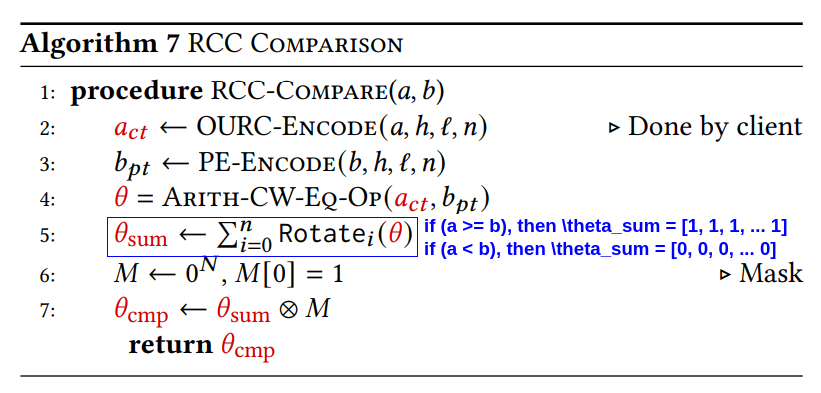
\includegraphics[width=0.7\linewidth]{figures/untitled.png}

\end{figure}

This figure shows the pseudo-code for the RCC-compare function that compares the size of $\alpha$ against $\beta$, and if $\alpha \geq \beta$, the function returns 1; otherwise, it returns 0. Inside this function, $\vec\theta$ contains an array of SumPath results where each slot is the equality check result (1 or 0) in each depth of the RCC comparison tree (i.e., complete binary tree). If any slot in $\vec\theta$ contains 1, this implies that $\alpha \geq \beta$ (i.e., $\alpha$ falls within the range of $[\beta, 2^n-1]$). If all slots in $\vec\theta$ contains 0, this implies that $\alpha < \beta$ (i.e., $\alpha$ falls outside of the range $[\beta, 2^n-1]$). 

In line 6, $\vec\theta_{\text{sum}}$ stores the aggregation of all possible rotations of $\vec\theta$ so that if $\vec\theta$ contains 1 in any slot, then $\vec\theta_{\text{sum}}$ ends up with $(1, 1, 1, \cdots, 1)$, whose number of slots is the depth of the RCC comparison tree. If $\vec\theta$ stores 0 for all slots, then $\vec\theta_{\text{sum}}$ ends up with $(0, 0, 0, \cdots, 0)$. 

When homomorphically evaluating the decision tree, all these computations are done as homomorphic addition and multiplication. Therefore, $\vec\theta$ and $\vec\theta_{\text{sum}}$ are encrypted as RLWE ciphertexts. That is, $\vec\theta_{\text{sum}}$ is encrypted as $\textsf{RLWE}_{S(X), \sigma}(\Delta M(X))$, where $M(X)$ is a polynomial that encodes the input. It can be that the input $(1, 1, 1, \cdots, 1)$ and $(0, 0, 0, \cdots, 0)$ are encoded into the following polynomials:

\(
    \vec\theta_{\text{sum}} =   
\begin{cases}
    (1, 1, 1, \cdots, 1) \rightarrow M(X) = 1 + 0X + 0X^2 + \cdots + 0X^{n-1} \\
    (0, 0, 0, \cdots, 0) \rightarrow M(X) = 0 + 0X + 0X^2 + \cdots + 0X^{n-1} \\
\end{cases}
\)

Remember that in the RLWE's batch encoding scheme, a polynomial $M(X)$ is decoded into a vector by evaluating $M(X)$ at $n$ different primitive $n$-th roots of unity: $\{x_0, x_1, x_2, \cdots, x_{n-1}\}$ (where each $x_i$ is a solution for $X^n + 1 \equiv 0 \bmod p$ and the order $\textsf{Ord}_p(x_i) = 2n$). Therefore, in order for the decoded vector $(M(x_0), M(x_1), M(x_2), \cdots, M(x_{n-1}))$ to be evaluated as $(1, 1, 1, \cdots, 1)$, the only possible polynomial $M(X) =1 + 0X + 0X^2 + \cdots + 0X^{n-1}$. Likewise, in order for the decoded vector to be $(0, 0, 0, \cdots, 0)$, the only possible polynomial $M(X) = 0 + 0X + 0X^2 + \cdots + 0X^{n-1}$. Therefore, we can conclude that if all slots of $\vec\theta_{\text{sum}}$ are 1, then $m_0 = 1$ (i.e., the constant term's coefficient of $M(X)$). And if all slots of $\vec\theta_{\text{sum}}$ are 0, then $m_0 = 0$.

Now, we will derive an LWE ciphertext that encrypts the 1st slot of $\vec\theta_{\text{sum}}$ (note that it does not matter which slot of $\vec\theta_{\text{sum}}$ we choose, because $\vec\theta_{\text{sum}}$ has the same value in all slots, anyway). According to the RLWE scheme, an RLWE ciphertext that encrypts $\Delta M(X)$ is structured as follows:  

$\textsf{RLWE}_{S(X), \sigma}(\Delta M(X)) = (A(X), B(X))$

, where $A(X) \in \mathcal{R}_{\langle n, q \rangle}$, \text{ } $B(X) = A(X) \cdot S(X) + \Delta M(X) + E(X) \text{ } \in \mathcal{R}_{\langle n, q \rangle}$

$ $


,where $A(X) = a_0 + a_1X^1 + a_2X^2 + \cdots + a_{n-1}X^{n-1} \text{ } \in \mathcal{R}_{\langle n, q \rangle}$

$B(X) = b_0 + b_1X^1 + b_2X^2 + \cdots + b_{n-1}X^{n-1} \text{ } \in \mathcal{R}_{\langle n, q \rangle}$

$E(X) = e_0 + e_1X^1 + e_2X^2 + \cdots + e_{n-1}X^{n-1} \text{ } \in \mathcal{R}_{\langle n, q \rangle}$

$S(X) = s_0 + s_1X^1 + s_2X^2 + \cdots + s_{n-1}X^{n-1} \text{ } \in \mathcal{R}_{\langle n, 2 \rangle}$

$ $

Remember our finding that all slots of $\vec\theta_{\text{sum}}$ has the value $m_0$ (i.e., $M(X)$'s constant term's coefficient). Now, we will derive the formula for $m_0$ based on the RLWE relation, as follows: 

$B(X) = A(X) \cdot S(X) + \Delta M(X) + E(X) \text{ } \in \mathcal{R}_{\langle n, q \rangle}$

$ $

$ b_0 + b_1X^1 + b_2X^2 + \cdots + b_{n-1}X^{n-1} = (a_0 + a_1X^1 + a_2X^2 + \cdots + a_{n-1}X^{n-1}) \cdot (s_0 + s_1X^1 + s_2X^2 + \cdots + s_{n-1}X^{n-1}) + \Delta \cdot (m_0 + m_1X + m_2X^2 + \cdots + m_{n-1}X^{n-1}) + (e_0 + e_1X^1 + e_2X^2 + \cdots + e_{n-1}X^{n-1})$

$ $

From the above relation, we extract the partial relation for the coefficients of the $X^0$ term as follows:

$b_0 = (s_0\cdot a_0) + \sum\limits_{i=1}^{n-1} (a_i\cdot s_{n - i}) + \Delta m_0 + e_0$

$= \sum\limits_{i=0}^{n-1}(a_i \cdot s'_i) + \Delta m_0 + e_0$ \textcolor{red}{\text{ } where $\vec{s'} = (s_0, s_{n-1}, s_{n-2}, \cdots, s_2, s_{1})$}

$= \textsf{LWE}_{\vec{s'}, \sigma}(\Delta m_0) = (\vec{a}, b_0)$ \textcolor{red}{\text{ } where $\vec{a}$ is a vector consisting of the coefficients of $A(X)$}

$ $

Notice that $\textsf{LWE}_{\vec{s'}, \sigma}(\Delta m_0)$ is an LWE ciphertext that encrypts the 1st slot of $\vec\theta_{\text{sum}}$. This last step of the RLWE-to-LWE conversion process is very fast, because we simply need to extract the coefficients of $A(X) and B(X)$ and combine them as vector components for an LWE ciphertext. 

We generalize the conversion of a batched RLWE ciphertext into LWE ciphertexts as follows. 

\begin{tcolorbox}[title={\textbf{Converting an Batched RLWE Ciphertext into LWE Ciphertexts}}]

Suppose RLWE's batch encoding process encodes the input $\vec{v} = (v_0, v_1, \cdots, v_{n-1})$ as the polynomial $M(X) = m_0 + m_1X + m_2X^2 + m_{n-1}X^{n-1}$, and encrypts as $\textsf{RLWE}_{S(X), \sigma}(\Delta M(X))$, which is structured as follows: 

$\textsf{RLWE}_{S(X), \sigma}(\Delta M(X)) = (A(X), B(X)) \text{ } \in \mathcal{R}_{\langle n, q \rangle}$

$A(X) = \sum\limits_{i=0}^{n-1} a_iX^i$, \text{ } $S(X) = \sum\limits_{i=0}^{n-1} s_iX^i$, \text{ } $E(X) = \sum\limits_{i=0}^{n-1} e_iX^i$

$B(X) = \sum\limits_{i=0}^{n-1} b_iX^i = A(X) \cdot S(X) + \Delta M(X) + E(X)$



$ $

We convert the RLWE ciphertext $\textsf{RLWE}_{S(X), \sigma}(\Delta M(X))$ as $n$ distinct LWE ciphertexts $\{\textsf{LWE}_{\vec{s'}, \sigma}(\Delta v_i)\}_{i=0}^{n-1}$ as follows:

\begin{enumerate}
\item We will first extract the $i$-th slot of $\vec{v}$ as an LWE ciphertext. To do this, we create a masking vector $\vec{k} = (0, 0, \cdots, 1, 0, 0, \cdots)$, which has 1 at the $i$-th position and 0s for all other positions. 

\item Compute $\vec{v}^{\langle K \rangle} = \vec{v} \cdot \vec{k}$. Therefore, $\vec{v}^{\langle K \rangle} = (0, 0, \cdots, v_i, 0, 0, \cdots)$

\item Compute $\vec{v}^{\langle R \rangle} = \sum\limits_{j=0}^{n-1} \textsf{Rotate}_j(\vec{v}^{\langle K \rangle})$. Therefore, $\vec{v}^{\langle R \rangle} = (v_i, v_i, \cdots, v_i, v_i)$. As an alternative version of this constant rotation, the number of rotations can be exponentially increased upon each addition (i.e., $1, 2, 4, \cdots$) to reduce the total number of required rotations from $n$ to $\log n$.   

\item Notice that $\textsf{LWE}_{\vec{s'}, \sigma}(\Delta m_0) = (\vec{a}, b_0)$ \text{ }, whose secret key $\vec{s'} = (s_0, s_{n-1}, s_{n-2}, \cdots, s_2, s_{1})$), and the masking vector $\vec{a}$ consists of the coefficients of the polynomial $A(X)$. 

\item We repeat the above steps for all $0 \leq i \leq n - 1$ to derive $n$ distinct LWE ciphertexts as follows: $\textsf{LWE}_{\vec{s'}, \sigma}(\Delta v_0), \text{ } \textsf{LWE}_{\vec{s'}, \sigma}(\Delta v_1), \cdots, \text{ } \textsf{LWE}_{\vec{s'}, \sigma}(\Delta v_{n-1})$.

\end{enumerate}



\end{tcolorbox}
\end{comment}

\begin{comment}

\clearpage

\subsection{XGBoost Homomorphic Inference}
\label{subsec:xgboost-homomorhpic}


\begin{figure}[!h]
    \centering
    \subfloat[Arithmetic Constant Weight Equality Comparison \href{https://arxiv.org/pdf/2309.06496}{(Source)}]{
  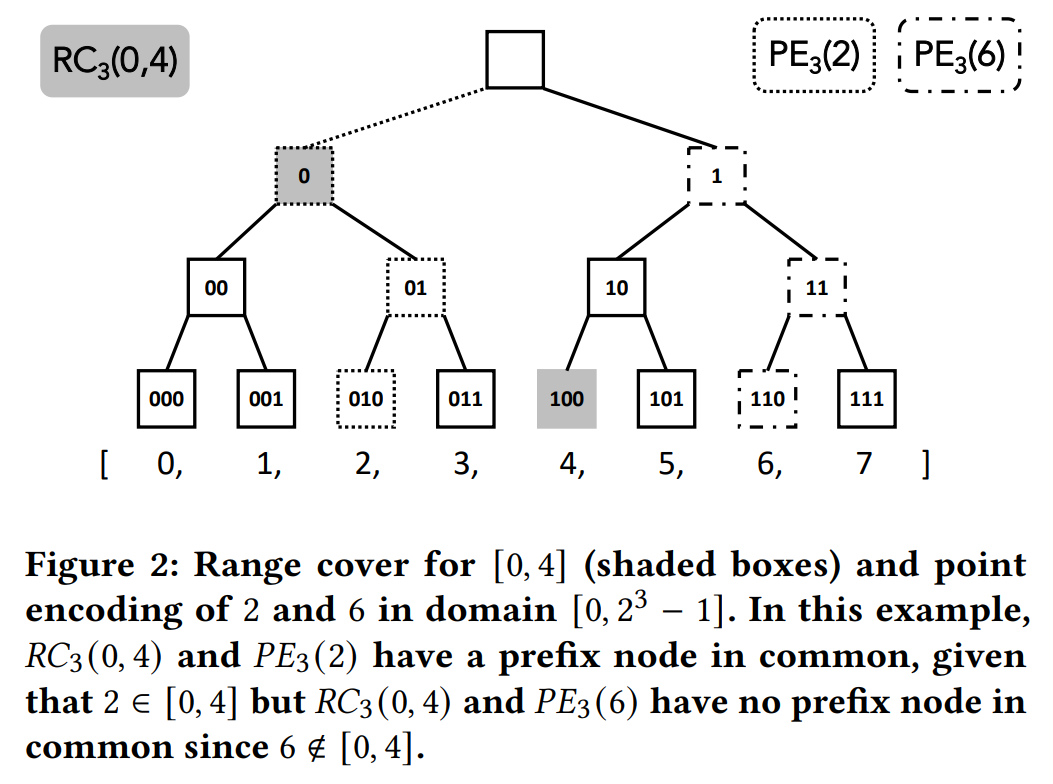
\includegraphics[width=0.5\linewidth]{figures/xgboost-2.png}

  \label{fig:encoding-tree}
}
    \subfloat[Binary Tree for RCC Comparison \href{https://arxiv.org/pdf/2309.06496}{(Source)}]{
  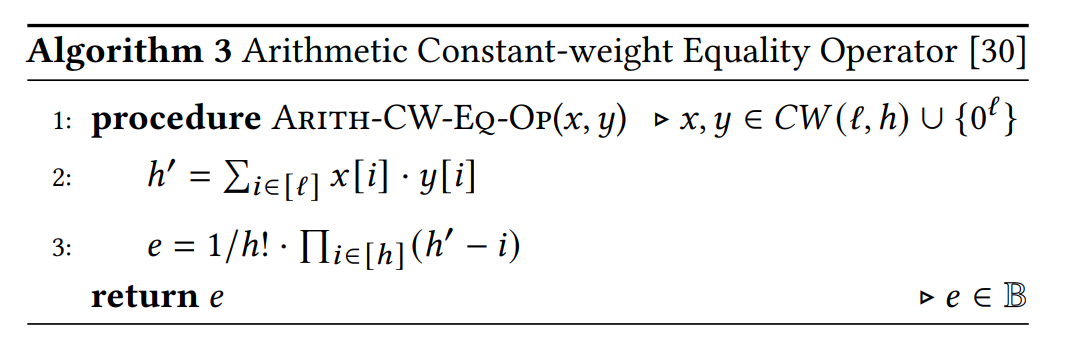
\includegraphics[width=0.5\linewidth]{figures/xgboost-1.png}

  \label{fig:arith-algo}
}
  \caption{}
\end{figure}

\subsection{Preliminaries}
\label{subsec:xgboost-preliminaries}

\subsubsection{XGBoost}

Suppose we have have $K$ decision trees in XGBoost where each tree $\textsf{Tree}_k$ has the weight score $w_k$. We have total $H$ nodes (expected to be 1,000$\sim$10,000 on average) in all decision trees in the trained XGBoost, where each tree node is denoted as $\textsf{Node}_h$. Suppose $\textsf{Tree}_k$ has $j_k$ paths, and each path $\textsf{Path}_{k,j_k}$ has a leaf node which has the class label $\textsf{Class}_c \in \mathcal{C}$. Each $\textsf{Node}_h$ (except for the leaf node) has a left edge and a right edge, each of which is denoted as $\textsf{LEdge}_h$ $\textsf{REdge}_h$. 
In XGBoost, each edge $\textsf{*Edge}_h$ (i.e., $\textsf{LEdge}_h$ or $\textsf{REdge}_h$) belongs to one or more paths. If $\textsf{*Edge}_h$ belongs to $\textsf{Path}_{k,j_k}$, let's denote this as $\textsf{*Edge}_h \hookrightarrow \textsf{Path}_{k,j_k}$.
If $\textsf{Path}_{k,j_k}$'s leaf node has the class $\textsf{Class}_c$, let's denote this as $\textsf{Path}_{k,j_k} \hookrightarrow \textsf{Class}_c$.  

\subsubsection{RCC-PDTE}

Let $l$ be the length of the constant-weight code word of the feature and threshold values in each tree node. Let $d$ be the depth of the \textsf{RC} and \textsf{PE} encoding tree (\autoref{fig:encoding-tree}). 

Let $\mu_{h, w} \in \{0, 1\}$ be the return value of $\textsf{Node}_h$'s \textsf{Arith-Eq-Op} operation, which is the equality comparison result of the $w$-th constant-weight code word compared between the feature and the threshold. We define $\vec{\theta}$ as follows:

$ \vec{\theta} = (\overbrace{\mu_{\langle 1,1\rangle}, \mu_{\langle 1,2\rangle}, \mu_{\langle 1,3 \rangle}, \cdots, \mu_{\langle 1,d\rangle}}^{d \text{ slots }}, \text{ } \overbrace{1, 1, 1, \cdots, 1}^{d-1 \text{repetitions}}, \text{ } \overbrace{\mu_{\langle 2,1\rangle}, \mu_{\langle 2,2\rangle}, \mu_{\langle 2,3\rangle}, \cdots, \mu_{\langle 2,d\rangle}}^{d \text{ slots }}, \text{ } \overbrace{1, 1, 1, \cdots, 1}^{d-1 \text{repetitions}},$

\text{ } \text{ } \text{ } $ \text{ } \text{ } \overbrace{\mu_{\langle 3,1\rangle}, \mu_{\langle 3,2\rangle}, \mu_{\langle 3,3\rangle}, \cdots, \mu_{\langle 3,d\rangle}}^{d \text{ slots }}, \text{ } \overbrace{1, 1, 1, \cdots, 1}^{d-1 \text{repetitions}} \text{ } \cdots )$

$ $

Each $\mu_{\langle i, j \rangle} \in \{0, 1\}$. Let $\mu_i = \sum\limits_{j=1}^{d}\mu_{\langle i, j \rangle} \in \{0, 1\}$ be the RCC comparison result of $\textsf{Node}_i$. 

\subsubsection{Fully Homomorphic Encryption}


We define RLWE's plaintext slot rotation operation as follows:

$\textsf{Rotate}(\vec{v}, h)$ : rotate the plaintext slot vector  $\vec{v}$ by $h$ positions to the left

\subsection{Scheme}
\label{subsec:xgboost-scheme}


$ $

\begin{enumerate}



\item We homomorphically rotate $\vec{\theta}$ and aggregate the intermediate results as follows: 

$\vec{\theta}_{\text{all}} = \sum\limits_{i=-(d-1)}^{d-1} \textsf{Rotate}(\vec{\theta}, i)$

\text{ } \text{ } \text{ } $= (\overbrace{\mu_1, \mu_1, \mu_1, \cdots, \mu_1}^{d \text{ repetitions }}, \text{ } \overbrace{?, ?, ?, \cdots, ?}^{d-1 \text{ repetitions}}, \text{ } \overbrace{\mu_2, \mu_2, \mu_2, \cdots, \mu_2}^{d \text{ repetitions }}, \text{ } \overbrace{?, ?, ?, \cdots, ?}^{d-1 \text{ repetitions}}, \text{ } \overbrace{\mu_3, \mu_3, \mu_3, \cdots, \mu_3}^{d \text{ repetitions }}, \cdots )$

\text{ } \text{ } \text{ } $= \sigma^{-1}(M(X))$

$ $

, where each $'?'$ is a whatever garbage value that we do not care.

$ $

\item For each tree node $\textsf{Node}_h$ where $h \in \{0, 1, 2, \cdots H - 1\}$, we compute the steps 3 $\sim$ 6. 


\item Define $\vec{v}_{\text{mask}}$ as a vector that stores value 1 in between the $(h\cdot (2d-1))$-th to $(h\cdot (2d-1)+d)$-th slots and 0 in all other slots. Homomorphically compute $\vec{\theta}_{\text{all}} \cdot \vec{v}_{\text{mask}}$. For example, if $h = 0$ in the first iteration, we homomorphically compute:

$\vec{\theta}_{\text{all}} \odot \vec{v}_{\text{mask}} =  \vec{\theta}_{\text{all}} \odot (\underbrace{\overbrace{1, 1, 1,\cdots 1}^{d \text{ repetitions}},  \overbrace{0, 0, 0, \cdots 0}^{(n-d) \text{ repetitions}}}_{n \text{ slots}})$
$= (\underbrace{\overbrace{\mu_1, \mu_1, \mu_1, \cdots, \mu_1}^{d \text{ repetitions}}, \overbrace{0, 0, 0, \cdots 0}^{(n-d) \text{ repetitions}}}_{n \text{ slots}})$ 

$= \vec{\theta}_{\text{all}}^{\langle 1 \rangle}$ 

$ $

\item Homomorphically compute: 

$\vec{\theta}_{\text{all}}^{\langle 2 \rangle} = \sum_{i=0}^{\frac{n}{d}-1}\textsf{Rotate}(\vec{\theta}_{\text{all}}^{\langle 1 \rangle}, \text{ } i \cdot d) = (\overbrace{\mu_h, \mu_h, \mu_h, \cdots, \mu_h}^{n \text{ repetitions }})$  

$ $

\item Now  we have $\textsf{RLWE}_{S(X), \sigma}(\Delta M'(X)) = (A'(X), B'(X))$ such that: 

$B'(X) = A'(X) \cdot S(X) + M'(X) + E'(X)$ 

$M'(X) = \sigma(\vec{\theta}_{\text{all}}^{\langle 2 \rangle}) = \sum\limits_{i=0}^{n-1} m'_i X^i = m'_0$ \textcolor{red}{\text{ } \# since $\vec{\theta}_{\text{all}}^{\langle 2 \rangle}$ is either $(1, 1, 1, \cdots, 1)$ or $(0, 0, 0, \cdots, 0)$}

$A'(X) = \sum\limits_{i=0}^{n-1} a'_iX^i$, \text{ } $S(X) = \sum\limits_{i=0}^{n-1} s_iX^i$, \text{ } $E'(X) = \sum\limits_{i=0}^{n-1} e'_iX^i$

$B'(X) = \sum\limits_{i=0}^{n-1} b'_iX^i = A'(X) \cdot S(X) + \Delta M'(X) + E'(X)$

$ $

\item Notice that $\textsf{LWE}_{\vec{s'}, \sigma}(\Delta m'_0) = (\vec{a'}, b'_0)$, whose secret key $\vec{s'} = (s_0, s_{n-1}, s_{n-2}, \cdots, s_2, s_{1})$ and the masking vector $\vec{a'}$ consist of the coefficients of the polynomial $A'(X)$. Also, notice that $\textsf{LWE}_{\vec{s'}, \sigma}(\Delta m'_0) = \textsf{LWE}_{\vec{s'}, \sigma}(\Delta \mu_h)$ which we want. Store $\textsf{LWE}_{\vec{s'}, \sigma}(\Delta \mu_h)$ in $\textsf{Node}_h$.

$ $

\item Repeat from step 2 to here for each $h \in \{0, 1, \cdots H-1\}$. Then, we finally get $\textsf{Node}_h = \textsf{LWE}_{\vec{s'}, \sigma}(\Delta \mu_h)$
 

$ $

\item For each non-leaf edge $\textsf{Node}_h$, homomorphically compute: 

$\textsf{LEdge}_h = \textsf{Node}_h$

$\textsf{REdge}_h = 1 - \textsf{Node}_h$

$ $

So, each truly traversed edge gets 0, whereas each non-traversed edge gets 1. 



$ $
\item For XGBoost's each path $\textsf{Path}_{k,j_k}$, homomorphically add up its edge values to compute the path scores as follows:

$\textsf{PathScore}_{k,j_k} = \sum\limits_{\textsf{*Edge}_h \hookrightarrow \textsf{Path}_{k,j_k}} \textsf{*Edge}_h$

$ $

\item  
For each $\textsf{PathScore}_{k,j_k}$, programmably bootstrap it such that:


\[
\begin{cases}
\text{If } \textsf{PathScore}_{k,j_k} = 0, \text{ then } \textsf{PathFinalScore}_{k,j_k} \leftarrow w_k\\
\text{If } \textsf{PathScore}_{k,j_k} \neq 0, \text{ then } \textsf{PathFinalScore}_{k,j_k} \leftarrow 0\\
\end{cases}
\] 


\item Homomorphically compute the weight score of each class $c \in \mathcal{C}$ as follows:

$ $

$\textsf{ClassScore}_{c} = \sum\limits_{\textsf{Path}_{k,j_k} \hookrightarrow \textsf{Class}_c} \textsf{PathFinalScore}_{k,j_k}$

$ $

\item $\{\textsf{ClassScore}_{c}\}_{c \in \mathcal{C}}$ is the set of the final score of each class in XGBoost.% where XGBoost's inference result is $\textsf{ArgMax}_{c \in \mathcal{C}}(\textsf{ClassScore}_{c})$. 

\end{enumerate}

\end{comment}






